\documentclass{beamer}

\title{Argumentation among Agents:\\Review and Commentary}
\author{Grigore Costin-Teodor \quad Radu Ștefan-Octavian \\ Vasiliu Florin \quad Vintilă Eduard}
\date{}


\usetheme{Frankfurt}
\setbeamerfont{itemize/enumerate subbody}{size=\normalsize}

\usepackage{tikz}
\usetikzlibrary{arrows.meta}


\begin{document}

\maketitle


\section{Florin}

\begin{frame}
\frametitle{Introduction}
\begin{itemize}
\item Reference: Iyad Rahwan's \emph{Argumentation among Agents}, Chapter 5 in \emph{Multiagent Systems}, by G. Weiss. \pause
\item Our contribution: several new examples, and proofs for some merely stated claims. \pause
\item What is the author attempting to formalize? \pause
\item The philosopher's view of argumentation: the giving of claims in favor or against a statement that is open for debate.
\end{itemize}
\end{frame}

\begin{frame}
\frametitle{Prakken's framework, briefly}
\begin{itemize}
\item Idea: generalize common logics by admitting two kinds of inference rules -- \emph{strict} and \emph{defeasible}. \pause
\item An \emph{argumentation system} is a tuple \( (\mathcal{L}, \mathit{cont}, S, D) \). \pause
\item $\mathcal{L}$ is some ``logical language'' (must contain $\neg$). \pause
\item The function \[ \mathit{cont} : \mathcal{L} \rightarrow \mathcal{P(L)} \] generalizes negation. \pause
\item $S, D$ are respectively the sets of strict/defeasible inference rules.
\end{itemize}
\end{frame}

\begin{frame}
\frametitle{Prakken's framework, briefly}
\begin{itemize}
\item How does the $\mathit{cont}$ function generalize negation? \pause
\item If \( \varphi \in \mathit{cont}(\psi) \), then
  \begin{itemize}
  \item[--] if \( \psi \not\in \mathit{cont}(\varphi) \), then $\varphi$ is a \emph{contrary} of $\psi$;
  \item[--] if \( \psi \in \mathit{cont}(\varphi) \), then $\varphi$ and $\psi$ are \emph{contradictory}.
  \end{itemize} \pause
\item It is mandatory that \[ \neg\varphi \in \mathit{cont}(\varphi) \mbox{\quad and\quad } \varphi \in \mathit{cont}(\neg\varphi) \] for any formula $\varphi$.
\end{itemize}
\end{frame}

\begin{frame}
\frametitle{Prakken's framework, briefly}
\begin{itemize}
\item An \emph{argument} from a knowledge base $\mathcal{K}$ is defined similarly to a deduction in propositional logic. (The members of $\mathcal{K}$ play the role of the hypotheses.) \pause
\item Major difference: incorporation of the used inference rules. \pause
\item The complete framework contains a partial order on defeasible rules. Using it, arguments may be compared.
\end{itemize}
\end{frame}

\begin{frame}
\frametitle{Dung's model}
\begin{itemize}
\item Henceforth, an \emph{argumentation framework} will mean a finite directed graph \( (\mathcal{A}, \rightharpoonup) \), whose nodes are called ``arguments''. The adjacency relation is pronounced ``defeats''. \pause
\item Hence, for arguments $p$, $q$,\quad ``$p \rightharpoonup q$'' means ``$p$ defeats $q$''. \pause
\item Note how the structure of arguments is not taken into account anymore. \pause
\item Objective: define an ``acceptable'' argument.
\end{itemize}
\end{frame}

\begin{frame}
\frametitle{Dung's model}
\begin{figure}
\centering
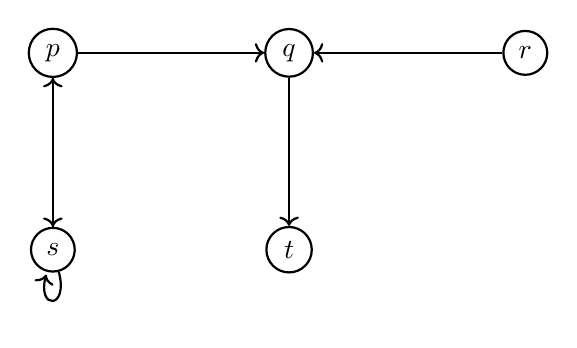
\begin{tikzpicture}
\tikzstyle{vertex} = [circle, draw=black, thick]
\tikzstyle{edge} = [->, thick]
\node[vertex] (p) at (0, 0) {$p$};
\node[vertex] (q) at (3, 0) {$q$};
\node[vertex] (r) at (6, 0) {$r$};
\node[vertex] (s) at (0, -2.5) {$s$};
\node[vertex] (t) at (3, -2.5) {$t$};
\draw[edge] (p)--(q);
\draw[edge] (p)--(s);
\draw[edge] (q)--(t);
\draw[edge] (r)--(q);
\draw[edge] (s)--(p);
\path (s) edge [loop below, thick] node {} (s);
\end{tikzpicture}
\caption{Our argumentation framework.} \label{af}
\end{figure}
\begin{itemize}
\item \( S^{+} = \mbox{ the set of arguments defeated by some member of } S \). \pause
\item In the figure, \( \{ p, q \}^{+} = \{ q, s, t \} \).
\end{itemize}
\end{frame}

\begin{frame}
\frametitle{Dung's model}
\begin{figure}
\centering
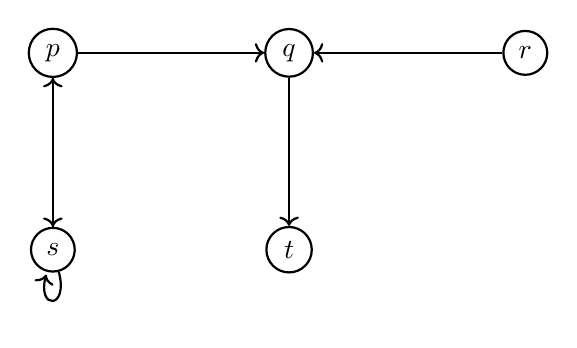
\begin{tikzpicture}
\tikzstyle{vertex} = [circle, draw=black, thick]
\tikzstyle{edge} = [->, thick]
\node[vertex] (p) at (0, 0) {$p$};
\node[vertex] (q) at (3, 0) {$q$};
\node[vertex] (r) at (6, 0) {$r$};
\node[vertex] (s) at (0, -2.5) {$s$};
\node[vertex] (t) at (3, -2.5) {$t$};
\draw[edge] (p)--(q);
\draw[edge] (p)--(s);
\draw[edge] (q)--(t);
\draw[edge] (r)--(q);
\draw[edge] (s)--(p);
\path (s) edge [loop below, thick] node {} (s);
\end{tikzpicture}
\caption{Our argumentation framework.} \label{af}
\end{figure}
\begin{itemize}
\item \( a^{-} = \mbox{ the set of arguments which defeat } a \). \pause
\item In the figure, \( s^{-} = \{ p, s \} \).
\end{itemize}
\end{frame}

\begin{frame}
\frametitle{Dung's model}
\begin{figure}
\centering
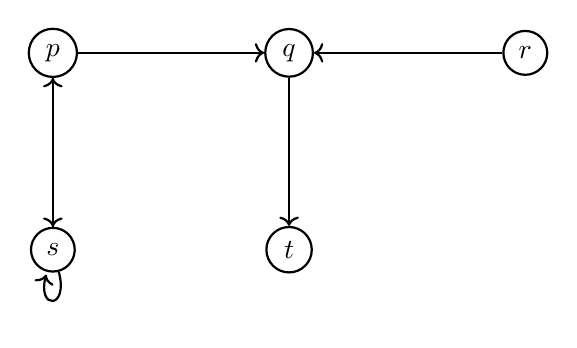
\begin{tikzpicture}
\tikzstyle{vertex} = [circle, draw=black, thick]
\tikzstyle{edge} = [->, thick]
\node[vertex] (p) at (0, 0) {$p$};
\node[vertex] (q) at (3, 0) {$q$};
\node[vertex] (r) at (6, 0) {$r$};
\node[vertex] (s) at (0, -2.5) {$s$};
\node[vertex] (t) at (3, -2.5) {$t$};
\draw[edge] (p)--(q);
\draw[edge] (p)--(s);
\draw[edge] (q)--(t);
\draw[edge] (r)--(q);
\draw[edge] (s)--(p);
\path (s) edge [loop below, thick] node {} (s);
\end{tikzpicture}
\caption{Our argumentation framework.} \label{af}
\end{figure}
\begin{itemize}
\item A set $S$ of arguments is \emph{conflict-free} if no argument in $S$ defeats another also in $S$. \pause
\item In the figure, $\{ p, t \}$ and $\{ r, t \}$ are conflict-free.
\end{itemize}
\end{frame}

\begin{frame}
\frametitle{Dung's model}
\begin{figure}
\centering
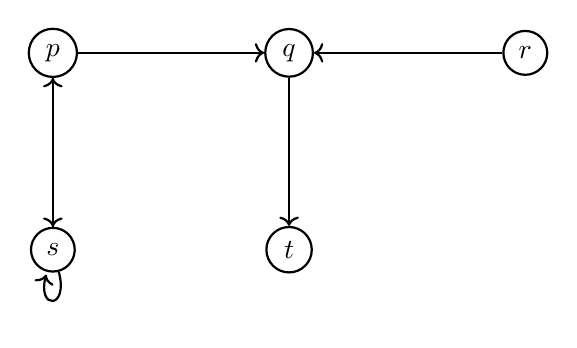
\begin{tikzpicture}
\tikzstyle{vertex} = [circle, draw=black, thick]
\tikzstyle{edge} = [->, thick]
\node[vertex] (p) at (0, 0) {$p$};
\node[vertex] (q) at (3, 0) {$q$};
\node[vertex] (r) at (6, 0) {$r$};
\node[vertex] (s) at (0, -2.5) {$s$};
\node[vertex] (t) at (3, -2.5) {$t$};
\draw[edge] (p)--(q);
\draw[edge] (p)--(s);
\draw[edge] (q)--(t);
\draw[edge] (r)--(q);
\draw[edge] (s)--(p);
\path (s) edge [loop below, thick] node {} (s);
\end{tikzpicture}
\caption{Our argumentation framework.} \label{af}
\end{figure}
\begin{itemize}
\item A set $S$ of arguments \emph{defends} argument $a$ if every argument which defeats $a$ is defeated by $S$ (i.e., is in $S^{+}$). \pause
\item In the figure, $\{ p, t \}$ defends $p$.
\end{itemize}
\end{frame}

\begin{frame}
\frametitle{Dung's model}
\begin{figure}
\centering
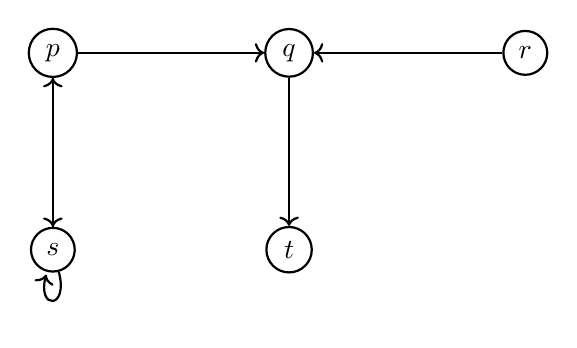
\begin{tikzpicture}
\tikzstyle{vertex} = [circle, draw=black, thick]
\tikzstyle{edge} = [->, thick]
\node[vertex] (p) at (0, 0) {$p$};
\node[vertex] (q) at (3, 0) {$q$};
\node[vertex] (r) at (6, 0) {$r$};
\node[vertex] (s) at (0, -2.5) {$s$};
\node[vertex] (t) at (3, -2.5) {$t$};
\draw[edge] (p)--(q);
\draw[edge] (p)--(s);
\draw[edge] (q)--(t);
\draw[edge] (r)--(q);
\draw[edge] (s)--(p);
\path (s) edge [loop below, thick] node {} (s);
\end{tikzpicture}
\caption{Our argumentation framework.} \label{af}
\end{figure}
\begin{itemize}
\item The \emph{characteristic function} $\mathcal{F}$ is defined thus:\\\centerline{\( \mathcal{F}(S) = \mbox{ the set of arguments defended by } S. \)} \pause
\item In the figure, \( \mathcal{F}(\{ p, q, r \}) = \{ p, r, t \} \) and \( \mathcal{F}(\{ r, t \}) = \{ r, t \} \).
\end{itemize}
\end{frame}

\begin{frame}
\frametitle{Dung's model}
\begin{figure}
\centering
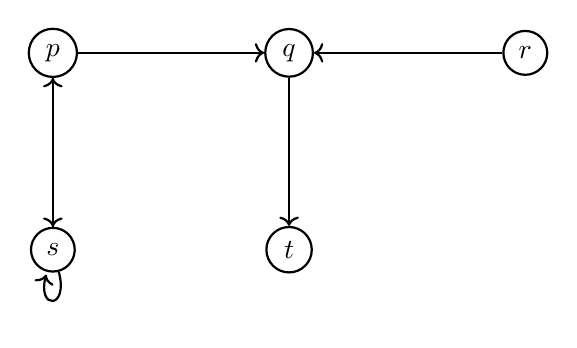
\begin{tikzpicture}
\tikzstyle{vertex} = [circle, draw=black, thick]
\tikzstyle{edge} = [->, thick]
\node[vertex] (p) at (0, 0) {$p$};
\node[vertex] (q) at (3, 0) {$q$};
\node[vertex] (r) at (6, 0) {$r$};
\node[vertex] (s) at (0, -2.5) {$s$};
\node[vertex] (t) at (3, -2.5) {$t$};
\draw[edge] (p)--(q);
\draw[edge] (p)--(s);
\draw[edge] (q)--(t);
\draw[edge] (r)--(q);
\draw[edge] (s)--(p);
\path (s) edge [loop below, thick] node {} (s);
\end{tikzpicture}
\caption{Our argumentation framework.} \label{af}
\end{figure}
\begin{itemize}
\item A \emph{complete extension} is a set $S$ of arguments which is conflict-free and such that \( \mathcal{F}(S) = S \) (i.e., it defends its own members and nothing else). \pause
\item By the remarks on previous slides, $\{ r, t \}$ is a complete extension.
\end{itemize}
\end{frame}

\begin{frame}
\frametitle{Dung's model}
\begin{itemize}
\item The author exhibits an equivalent characterization of complete extensions via \emph{labellings}. \pause
\item An argument $p$ is:
  \begin{itemize}
  \item[--] \emph{skeptically accepted}\quad iff $p$ belongs to every extension;
  \item[--] \emph{credulously accepted}\quad iff $p$ belongs to some extension;
  \item[--] \emph{rejected}\quad iff $p$ doesn't belong to any extension. 
  \end{itemize}
\end{itemize}
\end{frame}


\section{Eduard}

\section{Ștefan}

\begin{frame}{Strategic Argumentation \& Game Theory}
\begin{itemize}
    \item Background on the analysis of strategic argumentation
    \item Why Game Theory
    \item Important Game Theory Concepts
\end{itemize}
\end{frame}

\begin{frame}{Overview of strategic argumentation}
\begin{itemize}
    \item Various argumentation systems introduced. Each defines restrictions regarding what agents can and cannot do (e.g. Prakken's framework) \pause
    \item To analyze how a system behaves, one must also analyze the behaviour of agents, which will further be called ``strategy'' \pause
    \item Researchers started studying \emph{strategies} and how they affect the outcome of the argumentation \pause
    \item Parsons et al. introduce the \emph{dialogue system} based on \emph{attitudes} (e.g. confident, careful, thoughtful) \pause
    \item Other models based on \emph{social constructs} or \emph{mental states} are proposed by Nishan et al. and Kraus et al. \pause
\end{itemize}
\end{frame}

\begin{frame}{Why Game Theory}
\begin{itemize}
    \item Previous euristic approaches only consider a subset of all strategies \pause
    \item Game Theory provides a framework appropritate for a comprehensive analysis of \emph{strategic argumentation}\pause
    \item Can be used to achieve two goals:\pause
        \begin{itemize}
            \item predicting the outcome of a specific scenario\pause
            \item Designing a protocol such that a set of known agents behave
                in a desireable way (called \textbf{mechanism design})\pause
        \end{itemize}
\end{itemize}
\end{frame}

\begin{frame}{Glazer & Rubenstein's Model}
\begin{itemize}
    \item one of the first attempts of analyzing argumentation based on game theory
    \item \emph{procedural rules} (order and type of arguments) and \emph{persuation rules} (how the outcome is chosen / who wins the debate)
    \item no correlation between the logical structure of the information presented and the choice of the outcome
\end{itemize}
\end{frame}

\begin{frame}{Game Theory Concepts}
\begin{itemize}
    \item $I$ is the set of self-interested agents\pause
    \item $\theta_i \in \Theta$ is the type of agent $i$\pause
    \item $o \in \mathcal{O}$ is an outcome\pause
    \item utility function $u(o, \theta_i)$ defines \emph{how much} agent $i$ prefers outcome $o$\pause
    \item $s(\theta_i) \in \Sigma_i$ is a \emph{strategy} of agent $i$\pause
    \item $s=(s_1(\theta_1),\dots,s_I(\theta_I)) \in \mathcal{O}$ is a \emph{strategy profile}\pause
    \item for convenience:
        $s_{-i}(\theta_{-i}) = (s_1(\theta_1),\dots,s_{i-1}(\theta_{i-1}), s_{i+1}(\theta_{i+1}),\dots,s_I(\theta_I))$
        $\theta_{-i}=(\theta_1,\dots,\theta_{i-1},\theta_{i+1},\dots,\theta_I)$\pause
\end{itemize}
\end{frame}

\begin{frame}{Solution Concepts}
\begin{itemize}
    \item
\end{itemize}
\end{frame}

\section{Costin}


\end{document}
